\documentclass[pre,twocolumn,superscriptaddress,amsmath,amssymb]{revtex4-2}
\usepackage{graphicx}
\usepackage{bm}

\begin{document}

\title{Conditioning on estimated velocities: estimator artifacts in short-time Brownian motion}

\author{Luke Granto}
\affiliation{Independent researcher}

\date{Draft, 8 October 2026}

\begin{abstract}
Selecting trajectory segments by their initial velocity is a powerful way to expose short-time dynamics, but in practice the selected velocity is never instantaneous: it is a finite-difference estimate from time-averaged positions. We show that this changes what a velocity-conditioned mean-squared displacement (MSD) measures. For any stationary Gaussian process whose velocity autocorrelation has a short-time cusp, $C_v(\tau)=c-a|\tau|^{\alpha}$, the measured zero-velocity conditioned MSD separates into three parts. The first is the physical cusp term, distorted by a universal factor that depends only on $\alpha$, the stencil, and the lag in units of the averaging time. The second is a ballistic contribution leaking back through noise in the velocity estimate, whose size is given by an exact identity. The third is a constant noise floor. The distortion of the apparent exponent decays most slowly for soft cusps, which is precisely the hydrodynamic-memory case $\alpha=1/2$ in which a $t^{5/2}$ law has recently been reported. Applying the framework to the public data of that experiment, we find that the published hydrodynamic model is accurate. A calibration-free regression observable agrees with it to within 1.6\% from 0.75 to 192\,$\mu$s. Even so, the conditioned MSD is not a processing-independent quantity. In a preregistered test, recomputing velocity nine ways from the same positions changed the conditioned MSD by up to a factor of four, as a parameter-free forward model predicts ($\chi^2$-type statistic 20.9 over 32 cells, versus 4773 for the processing-independent reading). Over the same 3--12\,$\mu$s window the apparent exponent ranges from 2.29 to 2.96. The same mechanism makes stencil velocities appear smoother at short lags. It turns a passing value $H_v=1/4$ of the velocity roughness exponent into an apparent plateau when detector noise is not removed. We give a design criterion and remedies.
\end{abstract}

\maketitle

\section{Introduction}

Brownian motion in a liquid departs from the textbook Langevin picture at short times because the particle drags fluid with it: the Basset--Boussinesq history force gives the velocity autocorrelation a $t^{1/2}$ cusp and a long-time tail \cite{HaugeMartinLof1973,Hinch1975,Clercx1992}. High-bandwidth optical tracking has resolved the ballistic-to-diffusive transition, hydrodynamic resonances and the instantaneous velocity distribution \cite{Huang2011,Franosch2011,Kheifets2014}. A recent experiment \cite{Boynewicz2026} went further, selecting moments when the measured velocity is near zero and reporting that the subsequent MSD grows as $t^{5/2}$, a ``super-ballistic'' signature of the colored thermal force. Follow-up work discusses velocity-increment scaling with roughness exponent $H_v=1/4$ (fractal dimension $7/4$) \cite{FractalPreprint2026,PreparedPreprint2026}.

Both kinds of analysis condition on, or difference, an \emph{estimated} velocity. In practice positions are averaged over a bin of width $\Delta$ and velocity is a finite-difference stencil over several bins. The question we address is simple: how much of a velocity-conditioned statistic is the estimator? We derive a general answer, test it on the public data of Ref.~\cite{Boynewicz2026} \cite{Dryad2026} with protocols frozen before the confirmatory statistics were computed, and give a criterion for when the physical exponent is observable.

\section{Theory}

\subsection{Setup}

Let $x(t)$ be stationary and Gaussian with velocity autocorrelation
\begin{equation}
C_v(\tau)=c-a|\tau|^{\alpha}+o(|\tau|^\alpha),\qquad 0<\alpha\le 1,
\end{equation}
($\alpha=1/2$ for Basset memory, $\alpha=1$ for ordinary Langevin dynamics). The measured positions are bin averages $Y_n=\Delta^{-1}\int_{n\Delta}^{(n+1)\Delta}x\,dt$ and the velocity estimate is $W_n=\Delta^{-1}\sum_l d_l Y_{n+l}$ with a central stencil satisfying $\sum_l d_l=0$ and $\sum_l l\,d_l=1$. Selecting $W\approx 0$ and setting $D_k=Y_k-Y_0$, Gaussian conditioning gives the measured conditioned MSD
\begin{equation}
M_k=u_k-\frac{r_k^2}{s},\quad u_k=\mathrm{Var}\,D_k,\ r_k=\mathrm{Cov}(D_k,W),\ s=\mathrm{Var}\,W .
\end{equation}

\subsection{Three-term decomposition}

\emph{Cusp term.} The constant part $c$ of $C_v$ is ballistic motion, $x=v_0t$, for which $D_k=v_0k\Delta$ and $W=v_0$ exactly; its contribution to $M_k$ cancels identically. To first order in $a$, $M_k$ is therefore the variance of the residual functional $L_k=Y_k-Y_0-k\sum_l d_lY_l$, which annihilates constant and linear motion, evaluated with the generalized position covariance $\gamma(\tau)=a|\tau|^{\alpha+2}/[(\alpha+1)(\alpha+2)]$ (so that $-\gamma''=-a|\tau|^\alpha$). After bin averaging and scaling out $\Delta$,
\begin{equation}
M_k^{\rm cusp}=a\,\Delta^{\alpha+2}\,\Phi_\alpha(k),
\end{equation}
with $\Phi_\alpha$ a universal function of the lag in bins that depends only on $\alpha$ and the stencil. Its continuum limit $\Phi_\alpha\to 2k^{\alpha+2}/(\alpha+2)$ reproduces the instantaneous result $E[D^2|v_0=0]=2at^{\alpha+2}/(\alpha+2)$, i.e.\ $\tfrac45 a t^{5/2}$ for $\alpha=1/2$ \cite{Boynewicz2026}.

\emph{Ballistic leak.} Independent white position noise of variance $\sigma^2$ adds $\sigma_W^2=\sigma^2\sum_l d_l^2/\Delta^2$ to $s$ and, beyond the stencil reach, leaves $r_k$ unchanged. Exactly,
\begin{equation}
\delta M_k=2\sigma^2+\frac{\varepsilon}{1+\varepsilon}\,\frac{r_k^2}{s},\qquad \varepsilon=\frac{\sigma_W^2}{s}.
\end{equation}
Since $r_k^2/s\approx c\,t_k^2$ at short times, noise in the selection variable leaks a fraction $\varepsilon/(1+\varepsilon)$ of the ballistic $t^2$ term back into a quantity that should have cancelled it.

\emph{Floor.} The term $2\sigma^2$ is lag-independent.

The measured curve is thus a sum of terms with local exponents above $\alpha+2$ (the distorted cusp), equal to 2 (the leak) and equal to 0 (the floor).

\subsection{Universal distortion and a design criterion}

\begin{figure}[t]
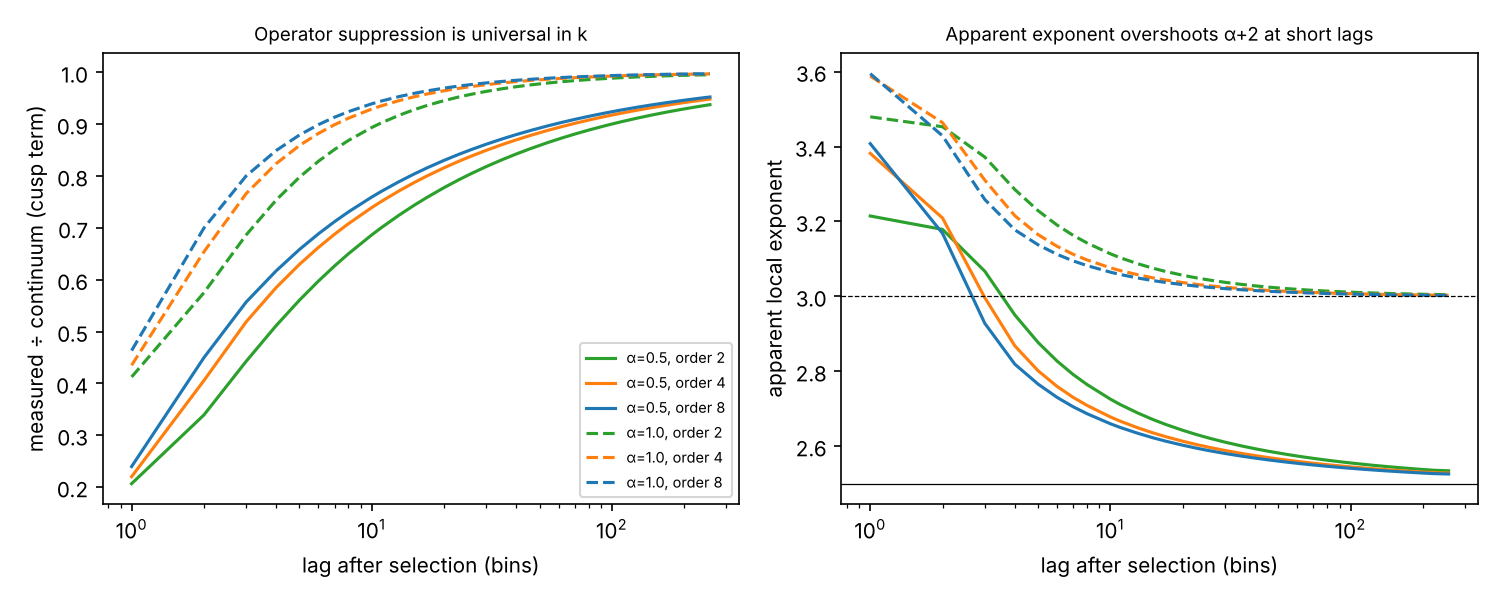
\includegraphics[width=\columnwidth]{figures/universal_operator_curves.png}
\caption{Universal estimator distortion of the cusp term. Left: $\Phi_\alpha(k)$ divided by its continuum limit. Right: apparent local exponent. Solid: $\alpha=1/2$; dashed: $\alpha=1$; stencils of order 2, 4, 8.}
\label{fig:universal}
\end{figure}

Figure~\ref{fig:universal} shows $\Phi_\alpha$. For $\alpha=1/2$ and an eighth-order stencil, the measured cusp term is 0.24, 0.62 and 0.82 of its continuum value at $k=1,4,16$. Its apparent exponent at $k=1$ is 3.41 rather than 2.5. The exponent is within 0.1 (0.05) of $\alpha+2$ only for $k\gtrsim 23$ (71) bins. For $\alpha=1$ the corresponding values are $k\gtrsim 7$ (13); for $\alpha=1/4$ the 0.1 threshold needs $k\gtrsim82$. Softer cusps, meaning stronger memory, recover most slowly. A clean $t^{\alpha+2}$ therefore requires all of the following:
\begin{itemize}
\item $t\gtrsim k_{\min}\Delta$, the operator condition;
\item $\varepsilon c t^2\ll at^{\alpha+2}$, the velocity-noise condition;
\item $2\sigma^2\ll at^{\alpha+2}$, the position-noise condition;
\item $t$ well below the onset of higher-order dynamics, for Basset memory $\min(\tau_f,\tau_p)$ with $\tau_f=\rho_f R^2/\eta$ and $\tau_p=m/6\pi\eta R$.
\end{itemize}
To first order in $a$ the theory agrees with the full Basset forward model (below) to within 1--5\% up to about 3\,$\mu$s at the parameters of Ref.~\cite{Boynewicz2026}. The leak identity is exact, and holds to machine precision numerically.

\subsection{Velocity roughness}

The same construction with weights $d_{l-k}-d_l$ gives $\mathrm{Var}(W_k-W_0)=a\Delta^\alpha\Psi_\alpha(k)$, with $\Psi_\alpha\to 2k^\alpha$. The apparent roughness exponent, half the local log-slope of $\Psi_\alpha$, is biased upward at short lags. For $\alpha=1/2$ (true $H_v=1/4$) with an eighth-order stencil it is 0.67, 0.50, 0.36, 0.31 and 0.29 at $k=1,2,4,8,16$: stencil velocities look smoother than the physical velocity.

\section{Application to public data}

We analyzed the six processed traces of Ref.~\cite{Dryad2026}: an optically trapped BaTiO$_3$ sphere in acetone ($R=3.40\,\mu$m), 750\,ns bins, an eighth-order stencil, and six empty-trap noise traces. All seven files matched their published SHA-256 digests. The authors' notebooks were read as text, not executed. Confirmatory protocols were committed before the corresponding real-data statistics were computed, each with synthetic positive and negative controls. Amendments are dated, and one inadvertent protocol deviation is disclosed (Methods).

\emph{The hydrodynamic model is accurate.} The regression slope $R_k=\mathrm{Cov}(D_k,W)/\mathrm{Var}\,W$, after subtracting empty-trap moments, has units of seconds and is independent of the volts-to-meters calibration. In equilibrium it equals the impulse response $m\chi(t)$ seen through the operator. With the published parameters and no free parameter, the Basset model matches $R_k$ to within 1.6\% from 0.75 to 192\,$\mu$s. A memoryless Langevin model with free damping and stiffness is rejected ($\Delta\chi^2=5483$). Equipartition through the operator reproduces the published calibration to 0.7--1.6\%; ignoring the operator gives an 8\% discrepancy. The power spectrum agrees with the model to 1--4\% from 2 to 100\,kHz (Fig.~\ref{fig:psd}).

\emph{The conditioned MSD is processing-dependent.} Through the published operator, the zero-velocity conditioned MSD of the Basset model is 0.26, 0.49, 0.67, 0.79 and 0.87 of the continuum curve at 0.75, 1.5, 3, 6 and 12\,$\mu$s. Empty-trap noise contributes an upper estimate of 71, 51, 27, 16 and 9\% of the measured value at the same lags. Over 0.75--6\,$\mu$s the log-log slopes are:
\begin{itemize}
\item operator alone: 2.93;
\item operator plus measured noise: 2.42;
\item data: 2.52;
\item continuum curve: 2.41.
\end{itemize}
To test this explanation we recomputed velocity from the supplied positions with stencils of order 2, 4 and 8, on positions coarsened by factors of 1, 2 and 4, giving nine variants. We compared ratios of conditioned MSDs to the published processing at 3, 6, 12 and 24\,$\mu$s; these ratios do not depend on the calibration. The forward model predicts ratios between 0.25 and 0.98. The processing-independent reading predicts 1. The frozen decision statistic was 20.9 for the forward model and 4773 for the processing-independent reading, over 32 cells. The median absolute log deviation from the forward model was 0.024, and the synthetic self-test returned the same verdict. Over 3--12\,$\mu$s the apparent exponent ranges from 2.29 to 2.96 with processing alone (Fig.~\ref{fig:processing}). At the published nonzero conditioning speeds the effect changes sign. Coarser processing suppresses the curve at $v_0=0.5\sigma$ and enhances it at $2\sigma$, both favoring the forward model, with a predicted crossover near $1\sigma$.

\begin{figure}[t]
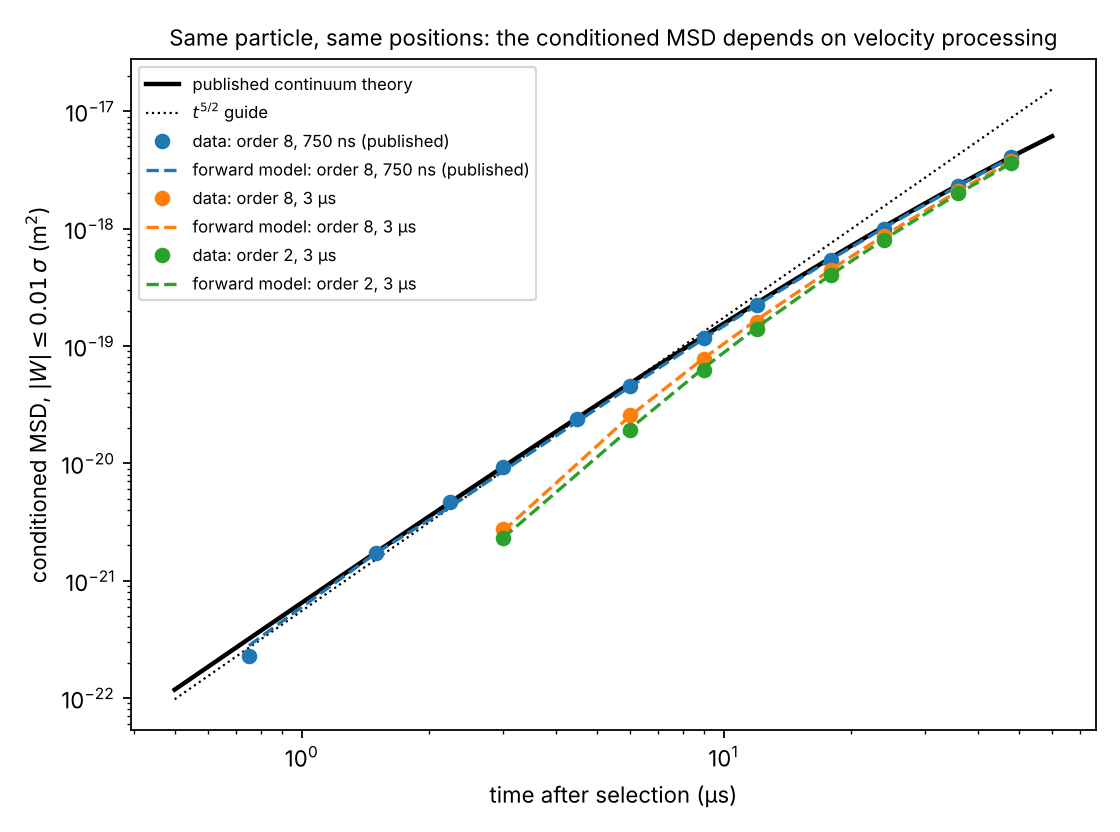
\includegraphics[width=\columnwidth]{figures/processing_dependence_figure.png}
\caption{Zero-velocity conditioned MSD from the same positions under three velocity estimators (points), the parameter-free forward model for each (dashed), and the continuum curve (solid). Only the published choice lands on the continuum curve.}
\label{fig:processing}
\end{figure}

\emph{Velocity roughness.} Noise-subtracted increment variances of recomputed stencil velocities follow the full Basset forward model to within 1--6\% beyond the fourth lag. In that model the local roughness exponent passes through $1/4$ near 11\,$\mu$s on its way down to the trap-dominated regime, and never plateaus. Without noise subtraction the data show an apparent plateau, $H_v\approx0.21$--0.25 over 1.5--12\,$\mu$s (Fig.~\ref{fig:roughness}), produced by detector noise flattening a falling curve. We could not read the velocity-roughness preprints \cite{FractalPreprint2026,PreparedPreprint2026} and do not know their estimator. We therefore state only that a plateau near $1/4$ in stencil-velocity increments is not, by itself, evidence of a scaling regime.

\begin{figure}[t]
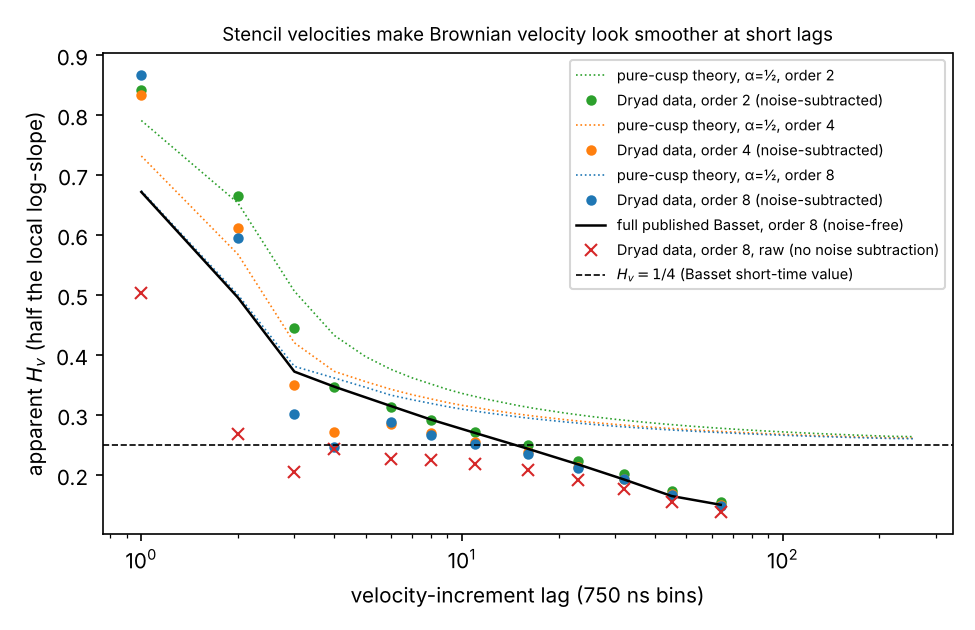
\includegraphics[width=\columnwidth]{figures/apparent_velocity_roughness.png}
\caption{Apparent velocity roughness exponent. Black: full Basset model through the published operator; dotted: first-order cusp theory; points: noise-subtracted data; crosses: raw data.}
\label{fig:roughness}
\end{figure}

\emph{Noise is not particle-independent.} Above 400\,kHz the particle traces are quieter than the empty-trap traces (Fig.~\ref{fig:psd}), so the noise floor with a particle present is roughly 0.5--0.7 of the empty-trap floor. Between 100 and 400\,kHz the particle spectrum exceeds model plus noise by about 23\%. This is the spectral counterpart of a 1--2\% structured residual in $R_k$ at 2--12\,$\mu$s. We could not resolve that residual with a free memory exponent, a detector low-pass, single- or two-component noise rescaling, or per-trace fits.

\begin{figure}[t]
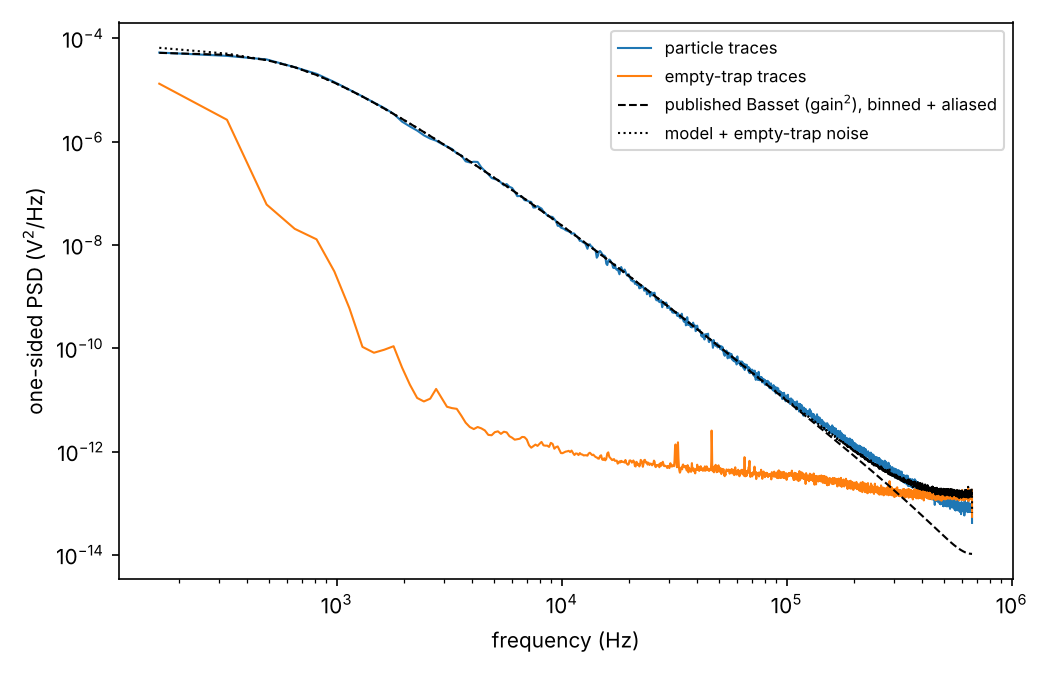
\includegraphics[width=\columnwidth]{figures/noise_additivity_psd.png}
\caption{Power spectra of particle and empty-trap traces with the published Basset spectrum (binned and aliased).}
\label{fig:psd}
\end{figure}

\section{Discussion}

Nothing here contradicts the hydrodynamics of Refs.~\cite{HaugeMartinLof1973,Hinch1975,Boynewicz2026}. The model is accurate. What changes is the evidential status of a plotted curve: a velocity-conditioned MSD built from estimated velocities is a property of the physics \emph{and} of the estimator. At the published settings its agreement with the continuum $t^{5/2}$ curve reflects two large effects that nearly cancel. The physical super-ballistic law is still recoverable, but only through a forward model or an estimator-independent observable such as $R_k$. Practical remedies are:
\begin{itemize}
\item model the operator and the noise explicitly;
\item report processing variants;
\item sample fast enough that $k_{\min}\Delta\ll\min(\tau_f,\tau_p)$; for this experiment $k_{\min}\Delta\approx17\,\mu$s while $\tau_f\approx28\,\mu$s, leaving essentially no clean window;
\item select on an independent velocity measurement, for example Doppler velocimetry, rather than on differences of the same positions.
\end{itemize}
The decomposition applies to any velocity-selected statistic, for instance in single-particle tracking and molecular dynamics.

\emph{Limitations.} The analysis covers one particle and one dataset, and the authors' upstream high-pass inversion was not varied. The theory is first order in $a$ and assumes stationary Gaussian statistics with white position noise; Fig.~\ref{fig:psd} shows the real noise is neither white nor particle-independent. A limited literature search found no prior treatment of this estimator effect, but we do not claim priority.

\section*{Methods and data availability}

All code, frozen protocols, results and digests are public in the repository \texttt{github.com/lukegranto23/physics-worldmap}: labs 34--47 under \texttt{Physics Worldmap/62 Computational Labs}, with write-ups as Benchmarks 014--018. Data are from Ref.~\cite{Dryad2026} (CC0) and are not redistributed. One disclosed protocol deviation concerns the calibration-free test: before its run, a rough first-lag value of $R/\Delta$ was computed while estimating noise levels from earlier saved results. No decision rule was changed.

\begin{acknowledgments}
We thank J.~Boynewicz, M.~C.~Thumann and M.~G.~Raizen for making their processed data and analysis notebooks public. The analysis and code were developed with assistance from an AI system (Claude, Anthropic); the author takes responsibility for the content.
\end{acknowledgments}

\begin{thebibliography}{99}
\bibitem{HaugeMartinLof1973} E.~H. Hauge and A.~Martin-L\"of, J. Stat. Phys. \textbf{7}, 259 (1973).
\bibitem{Hinch1975} E.~J. Hinch, J. Fluid Mech. \textbf{72}, 499 (1975).
\bibitem{Clercx1992} H.~J.~H. Clercx and P.~P.~J.~M. Schram, Phys. Rev. A \textbf{46}, 1942 (1992).
\bibitem{Huang2011} R.~Huang \emph{et al.}, Nat. Phys. \textbf{7}, 576 (2011).
\bibitem{Franosch2011} T.~Franosch \emph{et al.}, Nature \textbf{478}, 85 (2011).
\bibitem{Kheifets2014} S.~Kheifets, A.~Simha, K.~Melin, T.~Li, and M.~G. Raizen, Science \textbf{343}, 1493 (2014).
\bibitem{Boynewicz2026} J.~Boynewicz, M.~C. Thumann, and M.~G. Raizen, Sci. Adv. \textbf{12}, eaeb4579 (2026).
\bibitem{Dryad2026} J.~Boynewicz, M.~C. Thumann, and M.~G. Raizen, Dryad dataset, doi:10.5061/dryad.pvmcvdnz4 (2026).
\bibitem{FractalPreprint2026} ``The fractal dimension of Brownian dynamics in liquids,'' arXiv:2605.16252 (2026).
\bibitem{PreparedPreprint2026} ``Brownian motion: non-equilibrium states from equilibrium trajectories,'' arXiv:2605.16247 (2026).
\end{thebibliography}

\end{document}
